% coding:utf-8

%FOSAET, a LaTeX-Code for a electrical summary of basic electronics
%Copyright (C) 2013, Daniel Winz, Ervin Mazlagic

%This program is free software; you can redistribute it and/or
%modify it under the terms of the GNU General Public License
%as published by the Free Software Foundation; either version 2
%of the License, or (at your option) any later version.

%This program is distributed in the hope that it will be useful,
%but WITHOUT ANY WARRANTY; without even the implied warranty of
%MERCHANTABILITY or FITNESS FOR A PARTICULAR PURPOSE.  See the
%GNU General Public License for more details.
%----------------------------------------

\subsection{Subtrahierer / Differenzverstärker}
\begin{figure}[h!]
	\centering
	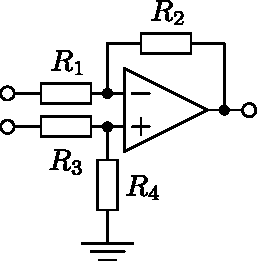
\includegraphics[scale=\schscale]{op_sub.pdf}
	\caption{Subtrahierer / Differenzverstärker}
	\label{sch:op-sub}
\end{figure}
\[ U_a = \frac{(R_1 + R_2) \cdot R_4}{(R_3 + R_4) \cdot R_1} \cdot U_{e+} 
- \frac{R_2}{R_1} \cdot U_{e-} \]
Wenn $R_1 = R_3$ und $R_2 = R_4$: 
\[ U_a = \frac{R_2}{R_1} \cdot (U_{e+} - U_{e-}) \]
Wenn $R_1 = R_2 = R_3 = R_4$: 
\[ U_a = U_{e+} - U_{e-} \]
\[ R_{e+} = R_3 + R_4 \]
\[ R_{e-} = R_1 \]
\[ R_a = 0 \]